% 第 21 题坐标图：按固定源 PDF 矢量路径换算（1 pt → 0.03515 cm）。
% 原点即两轴交点 O（源页 (1052.55, 260.43) pt），y 向上。椭圆半轴 70.84/50.09（比值 √2/2，与题设
% a=2、b=√2 同比例，按比例作图），线宽 0.8pt（源为其余图元 2 倍）；x 轴 −88.55..88.55、y 轴 ±70.84。
% 割线过 A、N、M、P 并向两端延伸（左越 A 15.6pt、右越 P 28.3pt）；竖直线 P–Q 垂直 x 轴；
% 弦 Q–B、A–B。M 为 PN 中点（源图自洽：M 在 y 轴上且为 PN 中点）。图上无实心圆点、坐标轴无刻度。
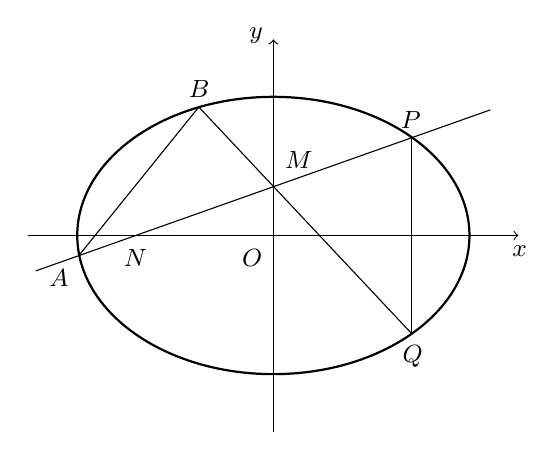
\begin{tikzpicture}[line cap=round,line join=round,font=\small,x=0.03515cm,y=0.03515cm]
% 坐标轴
\draw[->] (-88.55,0)--(88.55,0);
\draw[->] (0,-70.84)--(0,70.84);
% 椭圆（线宽 0.8，与源一致）
\draw[line width=0.8pt] (0,0) ellipse (70.84 and 50.09);
% 割线、竖直线 P–Q、弦 Q–B、弦 A–B
\draw (-85.71,-12.75)--(78.28,45.34);
\draw (49.94,35.42)--(49.94,-35.42);
\draw (49.94,-35.42)--(-26.92,46.40);
\draw (-70.13,-7.09)--(-26.92,46.40);
% ===== 标注（显式坐标，照源字形框中心）=====
\node[anchor=center,inner sep=0] at (-6.26,72.26) {\(y\)};
\node[anchor=center,inner sep=0] at (89.0,-5.59) {\(x\)};
\node[anchor=center,inner sep=0] at (-26.80,52.75) {\(B\)};
\node[anchor=center,inner sep=0] at (49.63,41.76) {\(P\)};
\node[anchor=center,inner sep=0] at (9.19,27.39) {\(M\)};
\node[anchor=center,inner sep=0] at (-49.78,-8.25) {\(N\)};
\node[anchor=center,inner sep=0] at (-7.60,-8.25) {\(O\)};
\node[anchor=center,inner sep=0] at (-77.40,-15.34) {\(A\)};
\node[anchor=center,inner sep=0] at (50.36,-43.68) {\(Q\)};
\end{tikzpicture}
